\section*{Anhang}
\addcontentsline{toc}{section}{Anhang}
\appendix
\startcontents[sections]
\printcontents[sections]{l}{1}{\setcounter{tocdepth}{2}}
\clearpage
\pagebreak


%\includepdf[pages={1},scale=0.95, pagecommand={\section{Anhangbsp mit PDF}},offset=0 -2cm]{sections/anhang/BA.pdf}
%\includepdf[pages={2-},scale=0.95, pagecommand={\thispagestyle{appendix}}]{sections/anhang/BA.pdf}

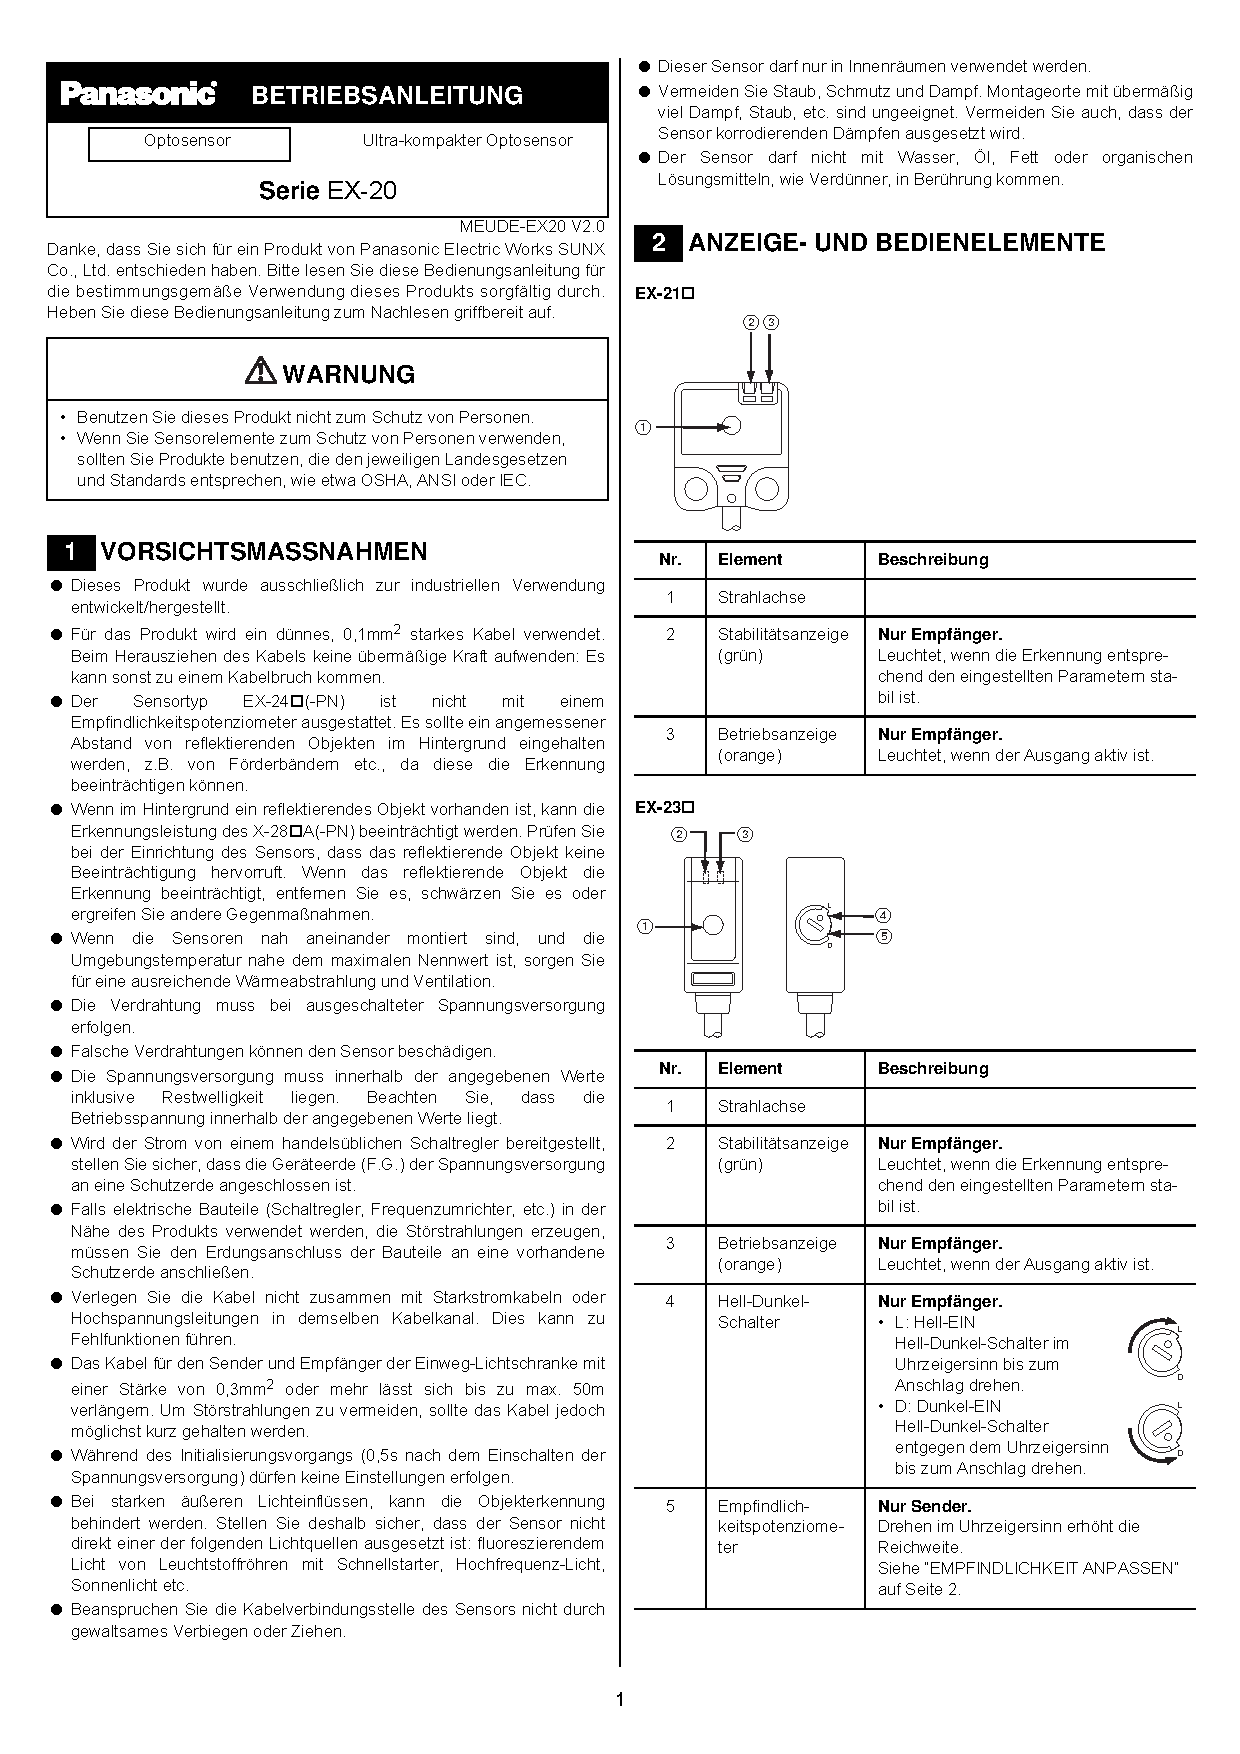
\includepdf[pages={1},scale=0.85, pagecommand={\section{Datenblatt Panasonic EX-20}\label{app:ex20}},offset=0 -2cm]{sections/anhang/ex20_ger_man.pdf}
\includepdf[pages={2-},scale=0.92, pagecommand={\thispagestyle{appendix}}]{sections/anhang/ex20_ger_man.pdf}


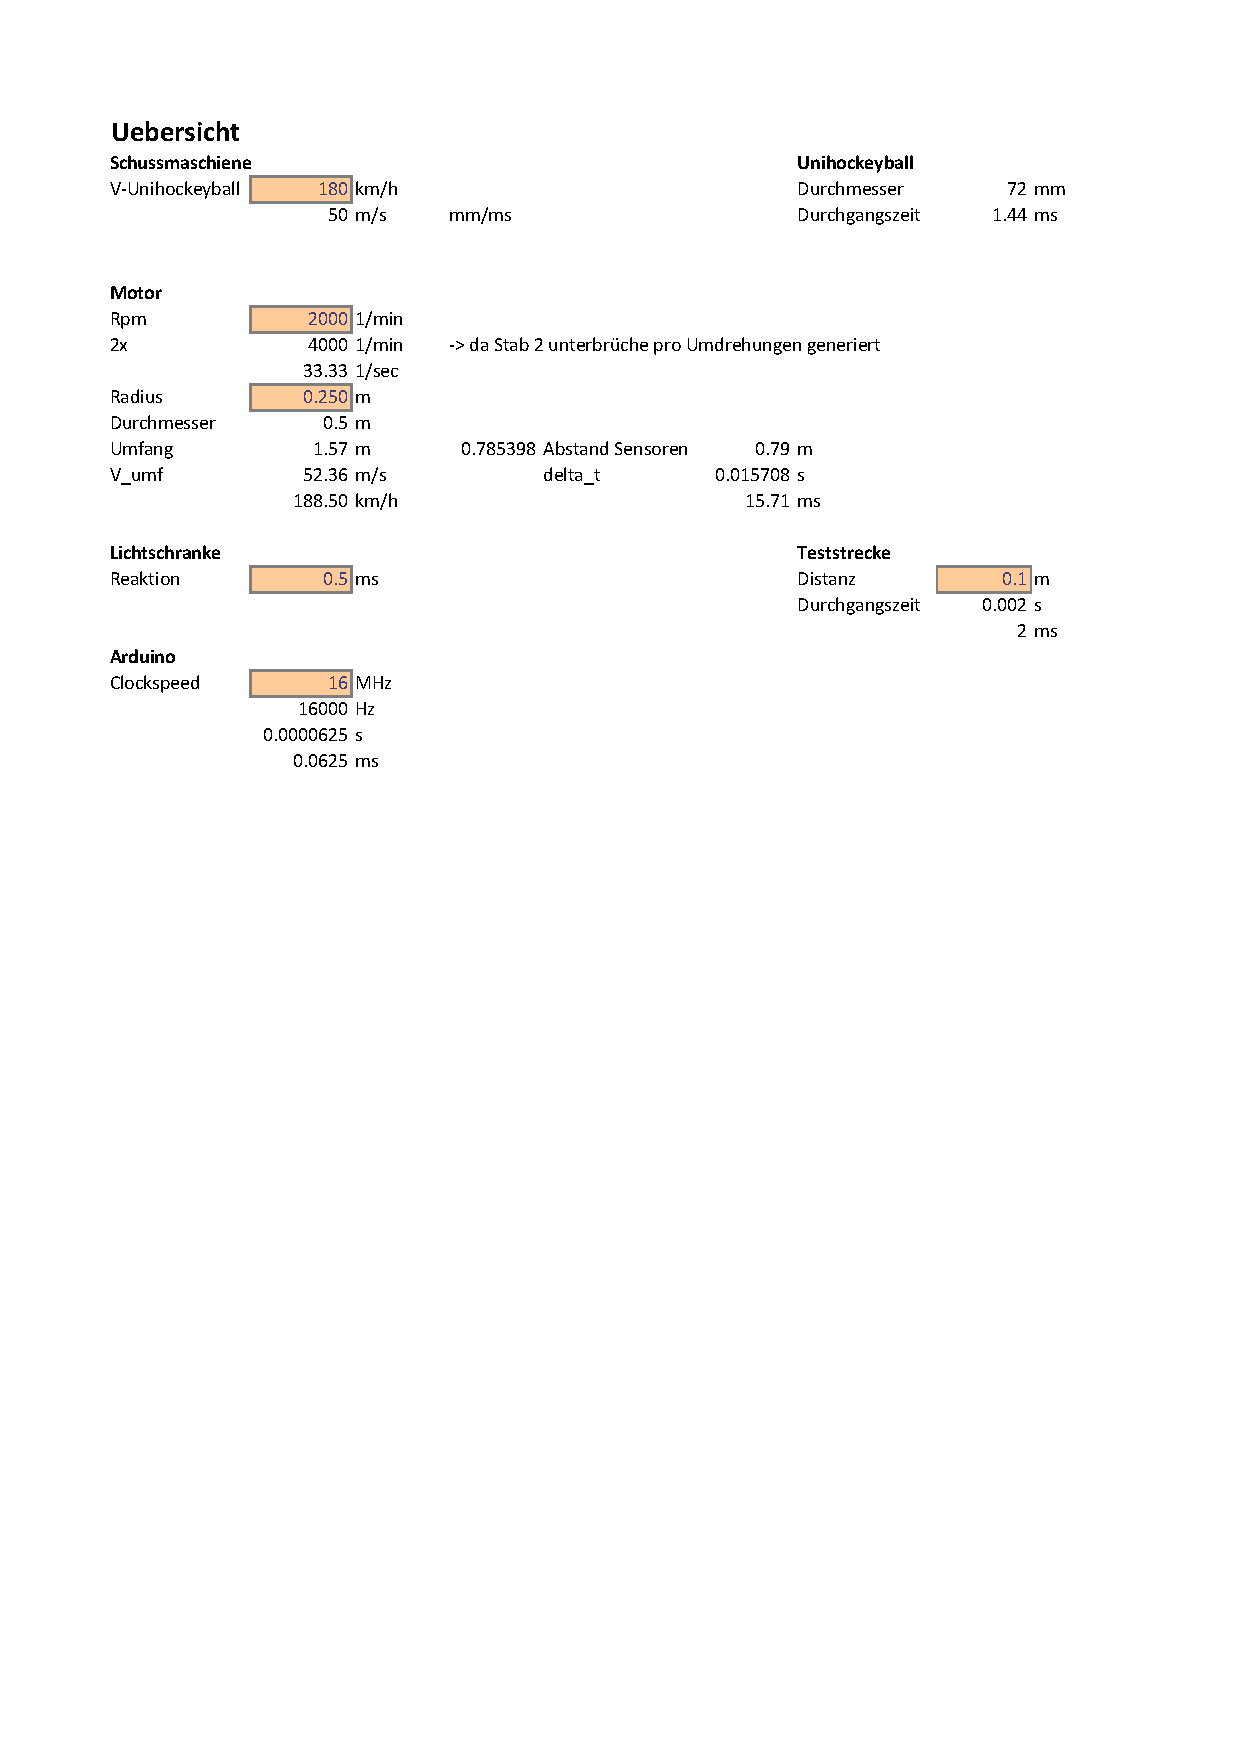
\includepdf[pages={1},scale=0.95, pagecommand={\section{Berechnungen}\label{app:berechnung}},offset=0 -2cm]{sections/anhang/Berechnungen.pdf}
\includepdf[pages={2,3},scale=0.95, pagecommand={\thispagestyle{appendix}}]{sections/anhang/Berechnungen.pdf}

\includepdf[pages={4},scale=0.95,
pagecommand={Für die Geschwindigkeit wird die Formel $\nicefrac{Umfang \cdot RPM}{60}$ angewendet. Die min/max Geschwindigkeit ergibt sich aus der Durchgangszeit $\pm$ des max. Sensorfehlers.
    \thispagestyle{appendix}},offset=0 -1.5cm]{sections/anhang/Berechnungen.pdf}
\includepdf[pages={5-},scale=0.95, pagecommand={\thispagestyle{appendix}}]{sections/anhang/Berechnungen.pdf}

\section{Arduinoprogramm}\label{app:ardprog}
\lstinputlisting[style=customc++]{src/BWMvelocity.cpp}
\clearpage
\section{Python}\label{app:python}
\lstinputlisting[style=python]{src/ReadSerial.py}
\clearpage
\section{Auswertung}\label{app:Auswertung}
\subsection{Matlab-skript}\label{app:matlab}
\lstinputlisting[style=custommatlab]{src/AuswertungHist.m}
\clearpage
\subsection{Plots}
\includegraphics[width=\textwidth]{images/auswertungLS1.png}\\
\includegraphics[width=\textwidth]{images/auswertungLS2.png}\\
\includegraphics[width=\textwidth]{images/auswertungLS1LS2.png}\\
\includegraphics[width=\textwidth]{images/auswertungInt.png}\\\


\includegraphics[width=\textwidth]{images/auswertungSpeedUeb.png}\\
\includegraphics[width=\textwidth]{images/auswertungSpeed.png}\\
\clearpage

\textbf{Gemessenens Signal bei 2000RPM}\newline
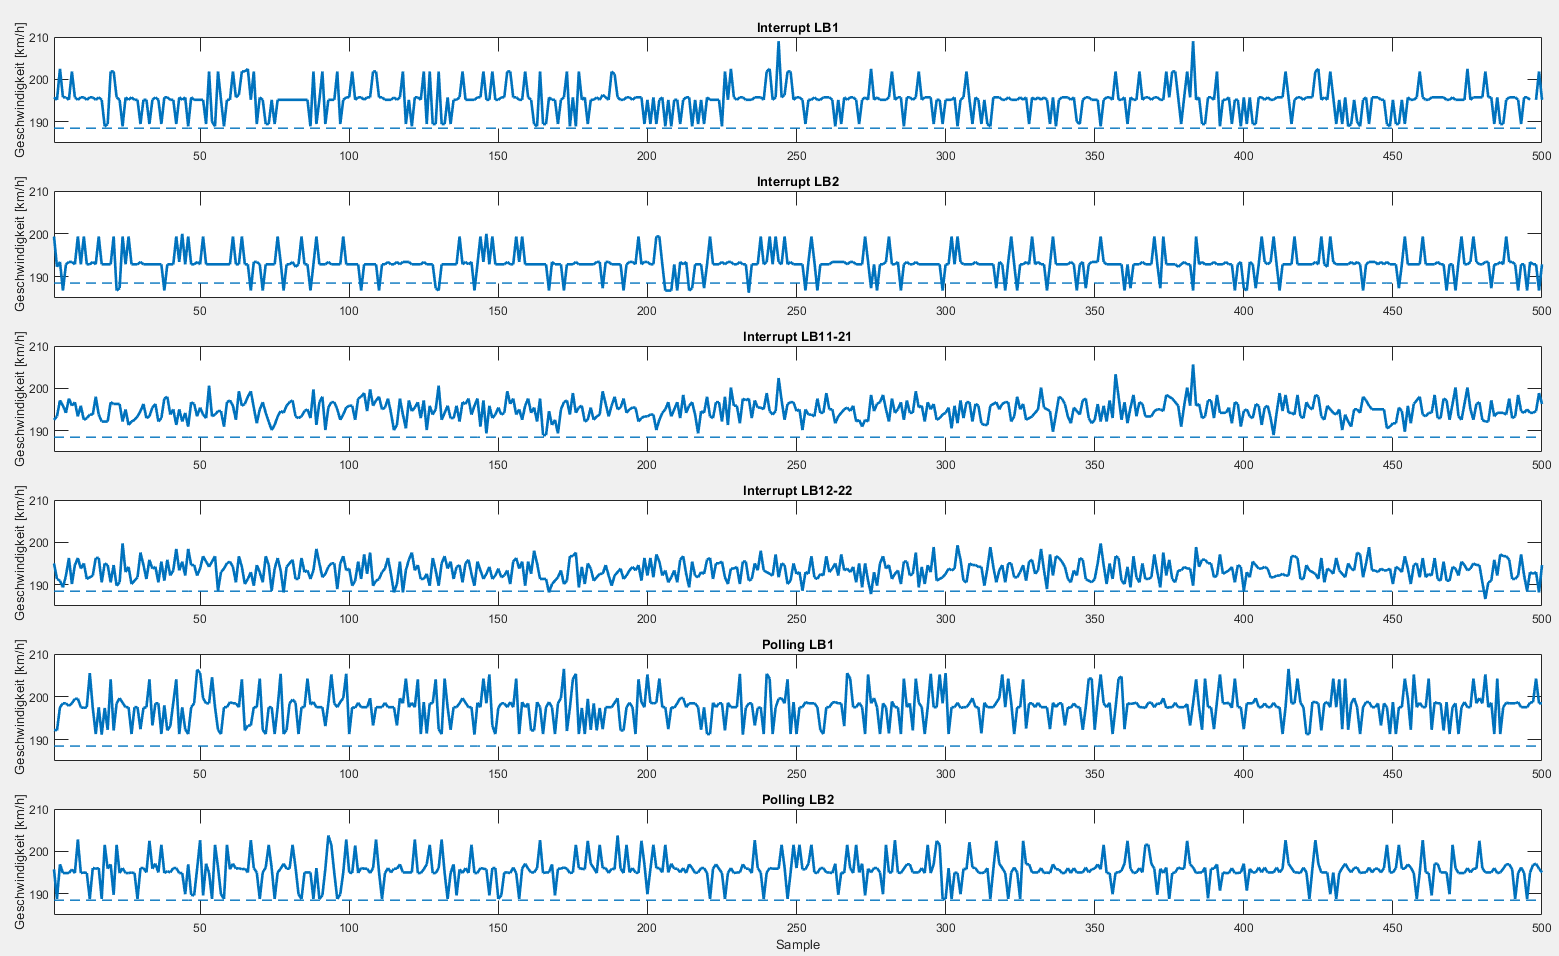
\includegraphics[width=\textwidth]{images/sig2000.png}\\

\textbf{Histogramm des gemessenen Signals bei 2000RPM}\newline
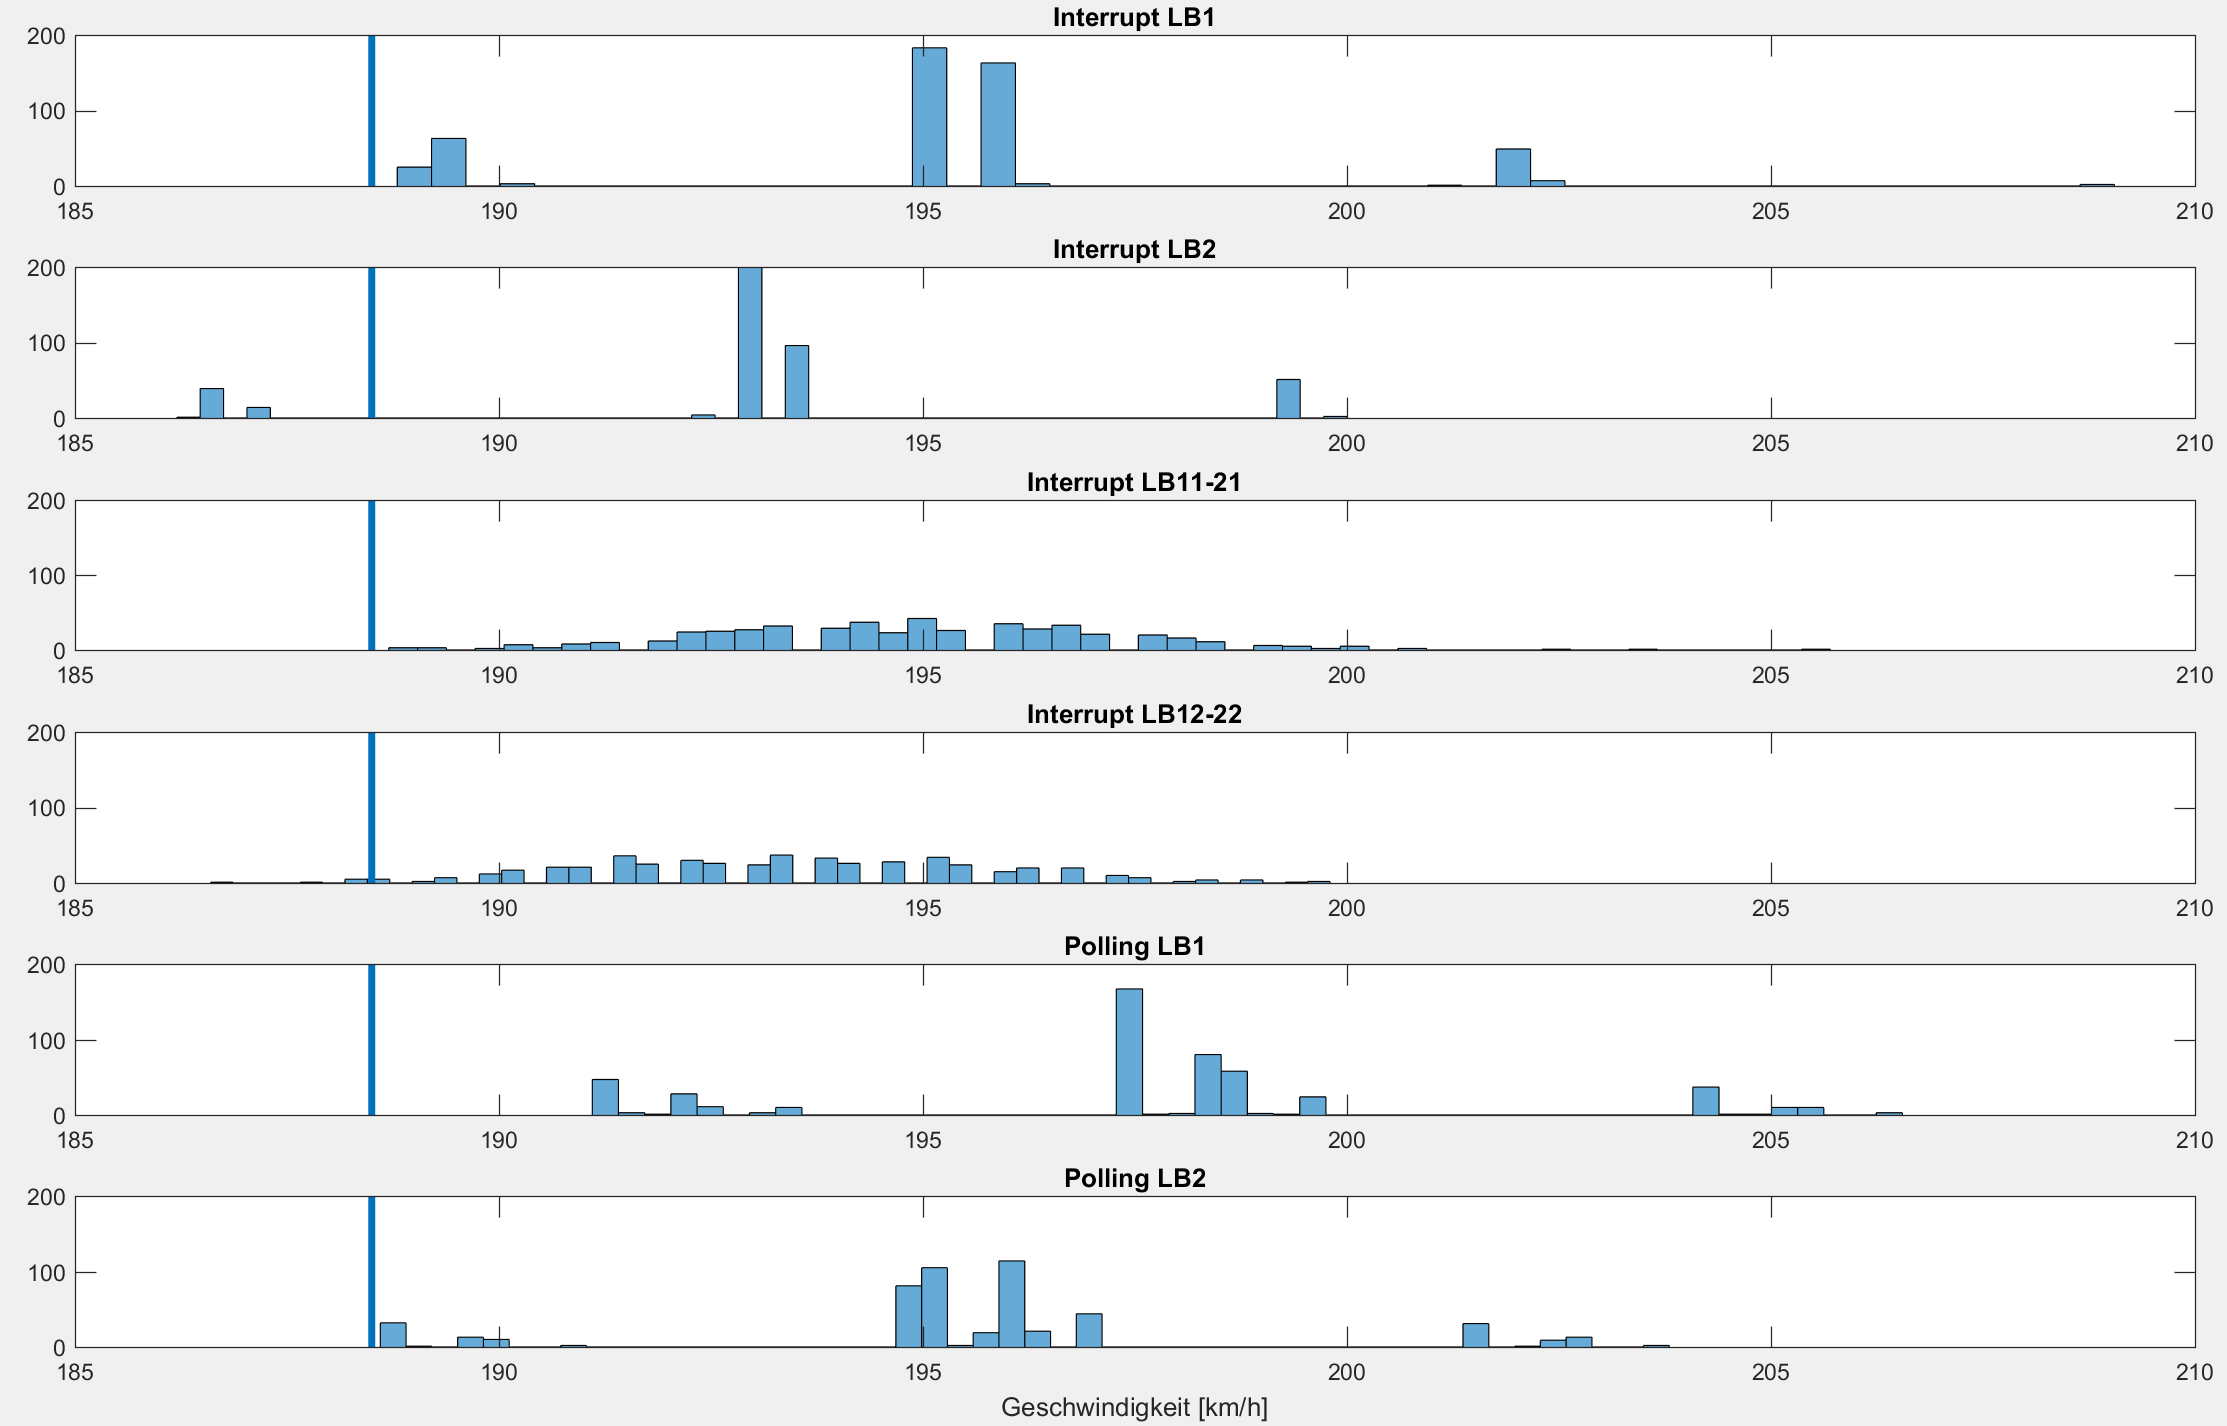
\includegraphics[width=\textwidth]{images/hist2000.png}
